%------------------------------------------------------------------------------
\chapter{Testing the impact of high and low energy hadronic interaction models for neutrino simulations}
\label{sec:app_2}
%------------------------------------------------------------------------------
This appendix contains an overview of the efforts done to check the dependence of the low and high hadronic interaction models used to simulate neutrino showers. The check was performed before the full library was simulated by the MC task. For the choice of the low energy hadronic interaction model UrQMD and FLUKA were compared and for the high energy model QGSJET-II-04,EPOS-LHC and SIBYLL 2.3d  were compared. The comparison was done by simulating 20 neutrino showers for each model for five different injected slant depths. The comparison was only done for $\nu_e$ CC showers with a primary energy of $10^{19}$eV for a zenith angle of $72^\circ$ was considered for the comparison. These three choices were made since such neutrinos are expected to give a good idea of the performance of the models and their effect to the overall analysis. The showers were simulated with CORSIKA 7.7.2 and the output was fed to the Offline analysis framework for the detector response simulation and reconstruction in the same way as described in chapter.~\ref{chap:DGL}. 

The comparison was done by calculating the ratio of the surviving events for both the models at each simulated slant depth. This comparison is shown in fig.~\ref{fig:Efficiency_vs_slant_comp_FLUKAnURQMD}. As seen in the figure the ration $\sim 1$ within the error bars which are high due to lack of statistics. After this comparison FLUKA was chosen as the main low energy hadronic model used in the simulations mainly because of ease of use. 

\begin{figure}[t!]
  \centering
  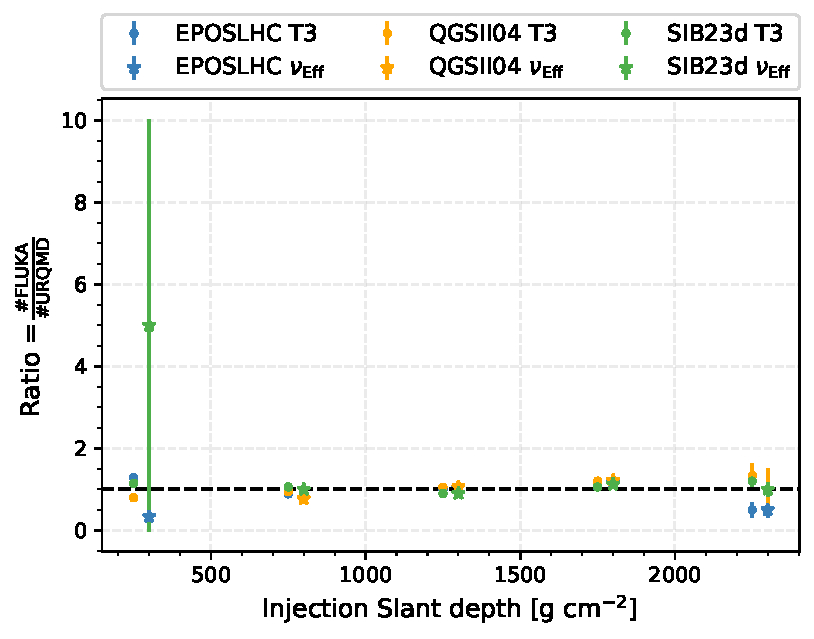
\includegraphics[width=\textwidth]{thesis_figures/App2/Efficiency_vs_slant_comp_FLUKAnURQMD.pdf}
  \caption{Ratio FLUKA vs URqmd}
  \label{fig:Efficiency_vs_slant_comp_FLUKAnURQMD}
\end{figure}

\begin{figure}[h!]
  \centering
  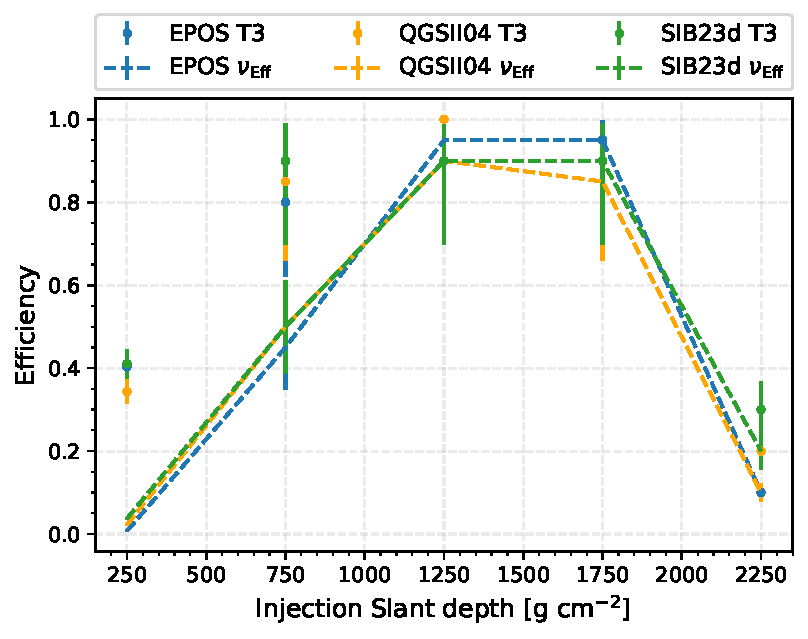
\includegraphics[width=\textwidth]{thesis_figures/App2/Efficiency_vs_slant_comp_all_HModel.pdf}
  \caption{All model eff comp}
  \label{fig:Eff_vs_slant_comp_all_HModels}
\end{figure}


For the choice of high energy interaction model The T3 and $\nu$ identification efficiency was calculated. The T3 efficiency was calculated as a ratio of the number of reconstructed events to the number of simulated events. The $\nu$ identification efficiency was not calculated according to the method presented in this thesis but rather with a less stringent cut where the AoP of the three earliest stations were required to be above 1.5. The efficiency was calculated relative to the total simulated events and was plotted against the different injected slant depths which were simulated. This was also done to attempt to calculate the systematic uncertainties which can arise due to the choice of the hadronic interaction model. The systematic uncertainties were calculated as the difference between the integral of efficiencies of the different models. Taking SIBYLL 2.3d as the reference model A, to test any other model the uncertainty is given by $\frac{\int A - \int B}{\int B}$. The results of the comparison are shown in fig.~\ref{fig:Eff_vs_slant_comp_all_HModels}. The calculated systematic uncertainties are below 5\% for the T3 efficiency and below 10\% for the $\nu$ identification efficiency. The relative uncertainty for the T3 efficiency for SIBYLL 2.3d in comparison to the EPOS-LHC was found to be $\sim +3\%$ and for QGSJETTII04 was found to be $\sim + 7\%$ and the uncertainty on $\nu$ identification was found to be $\sim +10\%$ for both the models. However, due to the limited statistics and the statistical errors being way higher ($\sim 20\%$) than the systematic differences no real differences were seen between the three models. However, a conservative choice of $\sim +5\%$ was chosen as systematic uncertainties related to the choice of the hadronic interaction model in this analysis by comparing with other sources mentioned before.  


